\newpage
{\bfseries IRSTI 61.13.17; 31.15.27}
\hfill {\bfseries \href{https://doi.org/10.58805/kazutb.v.2.23-456}{https://doi.org/10.58805/kazutb.v.2.23-456}}

\sectionwithauthors{N.U.Nurgaliyev, Ye.K.Aibuldinov,  Zh.B.Iskakova,A.Kolpek, T.T.Mashan, L.A.Kusepova, E.Ye Kopishev}{INVESTIGATION OF THE KINETICS OF THE COAL PYROLYSIS PROCESS}

\begin{center}
{\bfseries \textsuperscript{1,2} N.U.Nurgaliyev, \textsuperscript{1}Ye.K.Aibuldinov, \textsuperscript{1} Zh.B.Iskakova,\textsuperscript{3}A.Kolpek, \textsuperscript{3}T.T.Mashan, \textsuperscript{3}L.A.Kusepova, \textsuperscript{3}E.Ye Kopishev}

\textsuperscript{1} Research Institute of New Chemical Technologies,
L.N. Gumilyov Eurasian National University, Astana,

Kazakhstan,

\textsuperscript{2} Kazakh University of Technology and Business named
after K. Kulazhanov, Astana, Kazakhstan,

\textsuperscript{3} L.N. Gumilyov Eurasian National University, Astana,
Kazakhstan

Corresponding author: nurgaliev\_nao@mail.ru, elaman\_@mail.ru,
zhanariskakova@mail.ru
\end{center}

The study of the processes occurring in the temperature range of the
main decomposition of the organic mass of coal (OMC) makes it possible
to understand both the general patterns and the specifics of the
decomposition of solid fuels. This temperature interval is used to
calculate the kinetic parameters of the process, which carry important
information both about the nature of the structural-chemical
transformations and about the structure and direction of thermal
destruction of OMC. In this article, to study the kinetics of pyrolysis
of coal, the method of thermogravimetric analysis was used, in which
heating of coal samples was carried out in ceramic crucibles in the
temperature range of 25-900 °C at different heating rates (5-25 deg/min)
in nitrogen and oxygen media. Coal from the Kenderlyk deposit was chosen
as the object of study. Based on the constructed differential DTG curves
(dependence of the sample mass change rate on time) at different heating
rates, the kinetic parameters of pyrolysis of coal were calculated using
the equations of non-isothermal formal kinetics. The effect of the rate
and temperature of coal heating on the kinetic parameters of pyrolysis
of coal has been studied. The main stages of OMC decomposition are
revealed. It has been found that the heating rate of coal samples
significantly affects the temperature and process rate corresponding to
the main decomposition maxima on the differential DTG curves. The
dependence between the kinetic parameters of pyrolysis of coal in the
temperature range of the main decomposition of OMC on the rate and
temperature of heating, as well as between the kinetic parameters at
different stages of the main decomposition of coal, is analyzed.

{\bfseries Keywords:} thermogravimetric analysis, coal, pyrolysis, DTG
curves, kinetic parameters, decomposition stages, heating rate.

\begin{center}
{\large\bfseries ИССЛЕДОВАНИЕ КИНЕТИКИ ПРОЦЕССА ПИРОЛИЗА УГЛЯ}

{\bfseries \textsuperscript{1,2}Н.У.Нургалиев, \textsuperscript{1}Е.К.Айбульдинов, \textsuperscript{1}Ж.Б.Искакова, \textsuperscript{3}А.Колпек, \textsuperscript{3}Т.Т. Машан, \textsuperscript{3}Л.А.Кусепова, \textsuperscript{3} Э.Е. Копишев}

\textsuperscript{1}Научно-исследовательский институт Новых химических
технологий, Евразийский национальный университет им. Л.Н. Гумилева,
Астана, Казахстан,

\textsuperscript{2}Казахский университет технологии и бизнеса им. К.
Кулажанова, Астана, Казахстан,

\textsuperscript{3} Евразийский национальный университет им. Л.Н.
Гумилева, Астана, Казахстан,

e-mail: nurgaliev\_nao@mail.ru, elaman\_@mail.ru, zhanariskakova@mail.ru
\end{center}

Изучение процессов, протекающих в температурном интервале основного
разложения органической массы угля (ОМУ), позволяет понять как общие
закономерности, так и специфику разложения твердых топлив. Этот
температурный интервал используется для расчета кинетических параметров
процесса, которые несут важную информацию как о характере
структурно-химических превращений, так и о структуре и направлении
термодеструкции ОМУ. В данной статье для исследования кинетики пиролиза
угля использовали метод термогравиметрического анализа, в котором нагрев
образцов угля проводили в керамических тиглях в интервале температур
25-900°С при разных скоростях нагрева (5-25 град/мин) в средах азота и
кислорода. В качестве объекта исследования выбран уголь месторождения
Кендерлык. На основе построенных дифференциальных кривых DTG
(зависимость скорости изменения массы образца от времени) при разных
скоростях нагрева рассчитаны кинетические параметры пиролиза угля, с
использованием уравнений неизотермической формальной кинетики. Изучено
влияние скорости и температуры нагрева угля на кинетические параметры
пиролиза угля. Выявлены основные стадии разложения ОМУ. Установлено, что
скорость нагрева образцов угля заметно влияет на значения температуры и
скорости процесса, соответствующие максимумам основного разложения на
дифференциальных кривых DTG. Проанализирована зависимость между
кинетическими параметрами пиролиза угля в интервале температур основного
разложения ОМУ от скорости и температуры нагрева, а также между
кинетическими параметрами на разных стадиях основного разложения угля.

{\bfseries Ключевые слова:} термогравиметрический анализ, уголь, пиролиз,
кривые DTG, кинетические параметры, стадии разложения, скорость нагрева.

\begin{center}
{\large\bfseries КӨМІР ПИРОЛИЗІ ПРОЦЕСІНІҢ КИНЕТИКАСЫН ЗЕРТТЕУ}

{\bfseries \textsuperscript{1,2}Н.У.Нургалиев, \textsuperscript{1}Е.К.Айбульдинов, \textsuperscript{1}Ж.Б.Искакова, \textsuperscript{3}А.Колпек, \textsuperscript{3}Т.Т.Машан, \textsuperscript{3}Л.А.Кусепова, \textsuperscript{3} Э.Е. Копишев}

\textsuperscript{1}Жаңа химиялық технологиялар ғылыми-зерттеу институты,
Л.Н. Гумилев атындағы Еуразия ұлттық университеті, Астана, Қазақстан,

\textsuperscript{2}Қ.Құлажанов атындағы технология және бизнес
университеті, Астана, Қазақстан,

\textsuperscript{3}Л.Н. Гумилев атындағы Еуразия ұлттық университеті,
Астана, Қазақстан,

e-mail: nurgaliev\_nao@mail.ru, elaman\_@mail.ru, zhanariskakova@mail.ru
\end{center}

Көмірдің органикалық массасының (КОМ) негізгі ыдырауының температуралық
интервалында жүретін процестерді зерттеу қатты отындардың ыдырауының
жалпы заңдылықтарын да, ерекшеліктерін де түсінуге мүмкіндік береді. Бұл
температура аралығы құрылымдық-химиялық түрлендірулердің сипаты туралы
да, КОМ-ның термодеструкциясының құрылымымен бағыты туралыда маңызды
ақпаратты беретін процестің кинетикалық параметрлерін есептеу үшін
қолданылады. Бұл мақала да көмір пиролизінің термиялық деструкциясының
кинетикасын зерттеу үшін термогравиметриялық талдау әдісі қолданылды,
онда көмір үлгілерін қыздыру керамикалық тигельдерде азотпен оттегі
орталарында әртүрлі (5-25 градус/мин) қыздыру жылдамдығында 25-900 °С
температурада жүргізілді. Зерттеу объектісі ретінде Кендірлік кен
орнының көмірі таңдалды. Салынған DTG (үлгі массасының өзгеру
жылдамдығының уақытқа тәуелділігі) дифференциалдық қисықтар негізінде
әртүрлі қыздыру жылдамдықтарында көмір пиролизінің кинетикалық
параметрлері изотермиялық емес формальды кинетика теңдеулерін қолдана
отырып есептелді. Көмірді қыздыру жылдамдығымен температурасының пиролиз
процесінің кинетикалық параметрлеріне әсері зерттелді. КОМ-ның
ыдырауының негізгі кезеңдері анықталды. Көмір үлгілерінің қыздыру
жылдамдығы DTG дифференциалдық қисықтарындағы негізгі ыдырау
максимумдарына сәйкес келетін температурамен процесс жылдамдығының
мәндеріне айтарлықтай әсер ететіні анықталды. Көмір пиролизінің
кинетикалық параметрлері арасындағы тәуелсіздік, КОМ-нің негізгі ыдырау
температураларының аралығындағы қыздыру жылдамдығымен температурасына,
сондай-ақ көмірдің негізгі ыдырауының әртүрлі кезеңдеріндегі кинетикалық
параметрлер арасындағы байланыс талданады.

{\bfseries Түйін сөздер:}термогравиметриялық талдау, көмір, пиролиз, DTG
қисықтары, кинетикалық параметрлер, ыдырау кезеңдері, қыздыру
жылдамдығы.

\begin{multicols}{2}
{\bfseries Introduction.} When studying the kinetics of thermal
decomposition of solid fuels, the thermogravimetric analysis (TGA)
method is widely used, both in isothermal and dynamic modes {[}1-4{]}.
The express method of dynamic thermogravimetry has become widely used.
The proposed methods for determining the kinetic parameters of non
isothermal pyrolysis can be divided into model (model fitting) and
model-free, or isoconversion (model-free) {[}5{]}. When applying the
model method, it is sufficient to carry out one thermoanalytical
measurement. In the general case, the problem of determining the
constants is reduced to the selection and ``fitting'' of a mathematical
model for the reaction rate to the experimentally obtained kinetic curve
or its individual sections {[}6{]}. At the same time, kinetic analysis
using non-isoconversion methods does not allow one to evaluate the
dynamics of coal pyrolysis at different stages, since the resulting
total value of the apparent activation energy is a complex function of
the reactions occurring at individual stages.

Non-isothermal methods make it possible to obtain in a relatively short
time a great deal of information about the nature of the decomposition
process with registration of all transformation stages in a wide
temperature range. At the same time, the study of the processes
occurring in the temperature range of the main decomposition of the
organic mass of coal (OMC) makes it possible to understand both the
general patterns and the specifics of the decomposition of solid fuels.
This temperature interval is used to calculate the kinetic parameters of
the process, which carry important information both on the nature of
structural chemical transformations and on the structure and direction
of OMC thermal destruction {[}7{]}. At the same time, the composition
and properties of coal thermal processing products depend not only on
their structural and chemical characteristics, the nature of various
chemical additives, temperature, pressure, medium composition, but also
on the size of coal particles and the nature of heating (slow,
high-speed) {[}8{]}.

Mathematical models that are used to determine the kinetic parameters of
thermal degradation of coal cause certain difficulties due to their
complex structure, the variety of types of chemical bonds and
simultaneously occurring reactions {[}9,10{]}. Therefore, the choice of
an adequate kinetic model of thermal destruction is an important
research problem.

The purpose of this work is to study the kinetics of the pyrolysis of
coal using the TGA method. Coal from the Kenderlyk deposit (Kazakhstan)
was chosen as the object of study. The objectives of the study are to
determine the main stages of OMC decomposition, to study the influence
of the rate and temperature of coal heating on the kinetics of pyrolysis
of coal.

{\bfseries Materials and methods.} The experiments were carried out on a
TGA4000 thermogravimetric analyzer. Standard test methods for the
analysis of coal according to ASTM D7582-12 "Standard Test Methods for
Proximate Analysis of Coal and Coke by Macro Thermogravimetric Analysis"
was used. Coal samples were heated in ceramic crucibles in the
temperature range of 25-900°C at different heating rates (5-25 deg/min)
in the presence of nitrogen and oxygen. The sample weight was 1 gram.
The experiments were carried out in two stages. At the 1st stage, the
temperature was raised from room temperature 25°C to 40°C and kept at
this temperature for 15 minutes to stabilize the temperature. At the
second stage, the test sample in crucibles with a closed lid was heated
from 40°C to 915±3°C. The heating rate in different experiments was set
at 5, 10, 15, 20, 25 °C/min. When the furnace is heated, the TGA device
weighs the closed crucibles at certain intervals and records the data in
a special program.

The initial data for calculating the kinetic parameters of the process
under study were taken from the data of a special program (on a
computer), which displays the values of the masses of coal samples (mg),
heating rate (°C/min), time (sec), temperatures (°C). These parameters
are fixed at certain intervals during the entire period of programmed
heating.

To characterize the process of pyrolysis of OMC, the following
indicators were chosen: mass loss of samples in various temperature
ranges; temperature T\textsubscript{max}, velocity v\textsubscript{max},
rate constant k\textsubscript{max} corresponding to the highest rate of
mass loss (i.e., the maxima of the main decomposition on the DTG curves
at the inflection points); pre-exponential factor k\textsubscript{0} and
activation energy E\textsubscript{act} related to the stages of the main
thermal decomposition of coal. Due to the diversity and complexity of
physicochemical transformations, these kinetic parameters describe not
certain reactions, but the overall processes of pyrolysis of OMC,
therefore they are considered as ``effective parameters'' of formal
kinetics {[}11{]}.

The kinetic parameters of the main thermal decomposition of OMC were
determined based on the equations of non-isothermal formal kinetics
{[}12{]}. The Arrhenius law is used as the initial equation, which
describes the dependence of the reaction rate constant (k) on
temperature:

\begin{equation}
k = k_{0}e^{- E/RT}
\end{equation}

where $k_{0}$ -- pre-exponential factor; $E$ --
activation energy; $Т$ -- absolute temperature.

Equation (1) can be represented in the differential form:

\begin{equation}
v= d\alpha/dt = f(\alpha)k_{0}e^{- E/RT}
\end{equation}

where $v$ -- process speed, $α$ -- OMC conversion rate, $f (α)$ -- conversion
function.

According to experimental data {[}11{]}, the processes of the main
thermal decomposition of coal proceed in the first order, so the
function $f (α) = 1 - α$. Then, using the logarithm, equation (2) is
transformed to the form:

\begin{equation}
\ln \left[ \frac{1}{1 - \alpha} \cdot \frac{d\alpha}{d\tau} \right] = \ln k_{o} - \frac{E}{RT}
\end{equation}

Equation (3) is a linear equation $y=b+a\cdot x$,
in which \(y = \ln \left[ \frac{1}{1 - \alpha} \cdot \frac{d\alpha}{dt} \right],\ b = lnk_{0},\ а
= -E, x = 1/RT\), which makes it possible to lay the experimental points
on a straight line, from the tangent of the angle of inclination of
which to the abscissa axis, the activation energy of the process can be
calculated, and from the segment cut off along the ordinate axis, the
pre-exponential.

To obtain reliable results, experimental data are calculated using the
least squares method, according to which the coefficients a and b are
equal:
\end{multicols}

\begin{equation}
a = \frac{n \sum_{i=1}^{n} x_{i} y_{i} - \sum_{i=1}^{n} x_{i} \sum_{i=1}^{n} y_{i}}{n \sum_{i=1}^{n} x_{i}^{2} - \left( \sum_{i=1}^{n} x_{i} \right)^{2}},\
b = \frac{\sum_{i=1}^{n} \left( y_{i} - a \sum_{i=1}^{n} x_{i} \right)}{n}
\end{equation}


The root-mean-square errors of determining a and b (and hence the
activation energy and pre-exponential) are calculated as:

\begin{equation}
S_{a} = \sqrt{\frac{\sum_{i=1}^{n} \left( y_{i} - ax_{i} - b \right)^{2}}{\left( n - 2 \right) \sum_{i=1}^{n} \left( x_{i} - x_{\text{ср}} \right)^{2}}},\
S_{b} = \sqrt{ \left( \frac{\sum_{i=1}^{n} \left( y_{i} - ax_{i} - b \right)^{2}}{n - 2} \right) \left( \frac{1}{n} + \frac{x_{\text{ср}}^{2}}{\sum_{i=1}^{n} \left( x_{i} - x_{\text{ср}} \right)^{2}} \right) }
\end{equation}


Based on (4), the activation energy and the pre-exponential are
determined:

\begin{equation}
E = \frac{\sum_{i=1}^{n} \ln \left( \frac{1}{1 - \alpha} \cdot \frac{d\alpha}{d\tau} \right) \cdot \sum_{i=1}^{n} \left( \frac{1}{RT} \right) - n \sum_{i=1}^{n} \ln \left( \frac{1}{1 - \alpha} \cdot \frac{d\alpha}{d\tau} \right) \cdot \frac{1}{RT} }{n \sum_{i=1}^{n} \left( \frac{1}{RT} \right)^{2} - \left( \sum_{i=1}^{n} \frac{1}{RT} \right)^{2}}
\end{equation}

\begin{equation}
k_{0} = \exp \left[ \frac{\sum_{i=1}^{n} \left( \ln \left( \frac{1}{1 - \alpha} \cdot \frac{d\alpha}{d\tau} \right) - a \sum_{i=1}^{n} \ln \frac{1}{RT} \right)}{n} \right]
\end{equation}

\begin{multicols}{2}
The calculation of the kinetic parameters of the pyrolysis of OMC using
the above equations (1-7) was carried out using the computer program
MathCAD, in which the initial data are: arrays of mass values (weights
of undecomposed coal), time, temperature, as well as the values of the
serial numbers of the start and end points decomposition stages on the
DTG kinetic curves and the number of these points.

Results and discussion. The characteristics of the coal from the
Kenderlyk deposit are shown in Table 1.
\end{multicols}

\begin{table}[H]
\caption*{Table 1 - Characteristics of coal from the Kenderlyk deposit}
\centering
\begin{tabular}{|llllllll|ll|}
\hline
\multicolumn{8}{|l|}{\multirow{2}{*}{Composition of coal, \%}} & \multicolumn{2}{l|}{\begin{tabular}[c]{@{}l@{}}heat of combustion,\\   (kcal/kg)\end{tabular}} \\ \cline{9-10}
\multicolumn{8}{|l|}{} & \multicolumn{1}{l|}{higher} & lower \\ \hline
\multicolumn{1}{|l|}{W\tsp{r}} & \multicolumn{1}{l|}{A\tsp{r}} & \multicolumn{1}{l|}{V\tsp{daf}} & \multicolumn{1}{l|}{C\tsp{daf}} & \multicolumn{1}{l|}{O\tsp{daf}} & \multicolumn{1}{l|}{H\tsp{daf}} & \multicolumn{1}{l|}{N\tsp{daf}} & Sdaf & \multicolumn{1}{l|}{Q\tsp{r}\tsb{в}} & Q\tsp{r}\tsb{н} \\ \hline
\multicolumn{1}{|l|}{10.43} & \multicolumn{1}{l|}{9.62} & \multicolumn{1}{l|}{41.37} & \multicolumn{1}{l|}{74.41} & \multicolumn{1}{l|}{18.82} & \multicolumn{1}{l|}{4.79} & \multicolumn{1}{l|}{1.57} & 0.41 & \multicolumn{1}{l|}{6203} & 5752 \\ \hline
\end{tabular}
\end{table}

\begin{multicols}{2}
Figure 1 shows the DTG curves of coal in a nitrogen atmosphere at
heating rates of 10-25 deg/min. When analyzing the curves, three stages
of the main decomposition of the organic mass of coal of the Kenderlyk
deposit were revealed on the differential DTG curves, where peaks with
maxima of the mass loss rate (inflection points) are observed.
\end{multicols}

\begin{figure}[H]
	\centering
	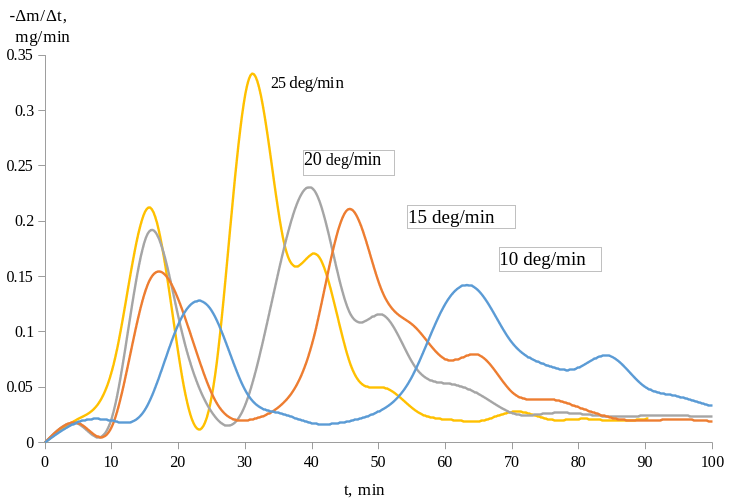
\includegraphics[width=0.6\textwidth]{assets/1085}
	\caption*{Figure 1 - DTG curves of coal in nitrogen environment}
\end{figure}

\begin{multicols}{2}
The first stage with a maximum at temperatures T\textsubscript{max} is
mainly associated with the release of oxygen-containing gases due to the
decomposition of side groups of macromolecules (because carbon-oxygen
bonds are the least thermally stable). At this stage, the bonds between
the main structural units are predominantly broken, side chains are
cleaved and partially decomposed, \emph{O\textsubscript{2}, N, S} are
partially removed. The yield of volatile substances in this temperature
range is low. In the 2\textsuperscript{nd} stagea peak is observed with
a maximum, which is responsible for the increase in the intensity of the
group of thermosynthesis reactions due to an increase in the reactivity
of the substances heated by the OMC. In this case, decomposition
reactions of hydroxyaromatic and heterocyclic fragments can occur, as
well as thermochemical transformations of humic substances and the
synthesis of new, more thermally stable compounds based on them, an
increase in the number of unsaturated bonds, and the rate of formation
of volatile substances increases {[}13{]}. At the third stage the
thermal decomposition reactions of the most thermally stable
organomineral complexes develop, by the end of this stage, the release
of the bulk of the resin and gaseous hydrocarbons is observed, the
process ends with the formation of semi-coke. With a further increase in
temperature, the aromatization and polycyclization reactions are
intensified (with the elimination of gaseous products, mainly
H\textsubscript{2}, and in a smaller amount, \emph{CH\textsubscript{4},
CO, N\textsubscript{2}}), and the formation of higher molecular
polycyclic systems of a network structure occurs.

At the 3rd stage of OMC decomposition at heating rates β from 10 to 25
deg/min, peaks with a maximum mass loss rate are weakly pronounced
(decreasing with increasing β), which is associated with the
superposition of several processes and the impossibility of their
separate estimates for the calculation of kinetic parameters (Figure 1).

Tables 2-5 show the results of calculating the kinetic parameters of the
pyrolysis of coal from the Kenderlyk deposit using the above method.
\end{multicols}

\begin{table}[H]
\caption*{Table 2 - Values of mass loss of coal samples and temperature T\textsubscript{max} at various stages of decomposition in a nitrogen environment}
\centering
\begin{tabular}{|l|llll|lll|}
\hline
\multirow{3}{*}{\begin{tabular}[c]{@{}l@{}}Speed of\\  heating,\\  °С /min\end{tabular}} & \multicolumn{4}{l|}{Mass loss from sample, \%} & \multicolumn{3}{l|}{Тmax, °С} \\ \cline{2-8}
 & \multicolumn{1}{l|}{\multirow{2}{*}{30-300°С}} & \multicolumn{1}{l|}{\multirow{2}{*}{300-600°С}} & \multicolumn{1}{l|}{\multirow{2}{*}{600-900°С}} & \multirow{2}{*}{30-900°С} & \multicolumn{3}{l|}{Stages of decomposition} \\ \cline{6-8}
 & \multicolumn{1}{l|}{} & \multicolumn{1}{l|}{} & \multicolumn{1}{l|}{} &  & \multicolumn{1}{l|}{1} & \multicolumn{1}{l|}{2} & 3 \\ \hline
5 & \multicolumn{1}{l|}{11.28} & \multicolumn{1}{l|}{18.74} & \multicolumn{1}{l|}{10.82} & \textit{40.84} & \multicolumn{1}{l|}{135} & \multicolumn{1}{l|}{347} & 461 \\ \hline
10 & \multicolumn{1}{l|}{10.27} & \multicolumn{1}{l|}{17.91} & \multicolumn{1}{l|}{9.71} & \textit{37.89} & \multicolumn{1}{l|}{161} & \multicolumn{1}{l|}{389} & 513 \\ \hline
15 & \multicolumn{1}{l|}{9.95} & \multicolumn{1}{l|}{17.23} & \multicolumn{1}{l|}{09.02} & \textit{36.20} & \multicolumn{1}{l|}{173} & \multicolumn{1}{l|}{402} & 547 \\ \hline
20 & \multicolumn{1}{l|}{9.52} & \multicolumn{1}{l|}{16.98} & \multicolumn{1}{l|}{8.94} & \textit{35.44} & \multicolumn{1}{l|}{192} & \multicolumn{1}{l|}{429} & 582 \\ \hline
25 & \multicolumn{1}{l|}{09.08} & \multicolumn{1}{l|}{16.15} & \multicolumn{1}{l|}{8.47} & \textit{33.70} & \multicolumn{1}{l|}{217} & \multicolumn{1}{l|}{443} & 621 \\ \hline
\end{tabular}%
\end{table}

\begin{table}[H]
\caption*{Table 3 - Values of mass loss of coal samples and temperature T\textsubscript{max} at various stages of decomposition in an oxygen environment}
\centering
\begin{tabular}{|l|llll|lll|}
\hline
\multirow{3}{*}{\begin{tabular}[c]{@{}l@{}}Speed of\\  heating,\\  °С/min\end{tabular}} & \multicolumn{4}{l|}{Mass loss from sample, \%} & \multicolumn{3}{l|}{Тmax, °С} \\ \cline{2-8}
 & \multicolumn{1}{l|}{\multirow{2}{*}{30-300°С}} & \multicolumn{1}{l|}{\multirow{2}{*}{300-600°С}} & \multicolumn{1}{l|}{\multirow{2}{*}{600-900°С}} & \multirow{2}{*}{30-900°С} & \multicolumn{3}{l|}{Stages of decomposition} \\ \cline{6-8}
 & \multicolumn{1}{l|}{} & \multicolumn{1}{l|}{} & \multicolumn{1}{l|}{} &  & \multicolumn{1}{l|}{1} & \multicolumn{1}{l|}{2} & 3 \\ \hline
5 & \multicolumn{1}{l|}{14.87} & \multicolumn{1}{l|}{23.72} & \multicolumn{1}{l|}{14.09} & \textit{52.68} & \multicolumn{1}{l|}{143} & \multicolumn{1}{l|}{364} & 467 \\ \hline
10 & \multicolumn{1}{l|}{13.92} & \multicolumn{1}{l|}{22.81} & \multicolumn{1}{l|}{13.26} & \textit{49.99} & \multicolumn{1}{l|}{170} & \multicolumn{1}{l|}{383} & 515 \\ \hline
15 & \multicolumn{1}{l|}{12.81} & \multicolumn{1}{l|}{21.79} & \multicolumn{1}{l|}{12.13} & \textit{46.73} & \multicolumn{1}{l|}{181} & \multicolumn{1}{l|}{420} & 532 \\ \hline
20 & \multicolumn{1}{l|}{11.59} & \multicolumn{1}{l|}{20.45} & \multicolumn{1}{l|}{11.27} & \textit{43.31} & \multicolumn{1}{l|}{208} & \multicolumn{1}{l|}{448} & 558 \\ \hline
25 & \multicolumn{1}{l|}{11.18} & \multicolumn{1}{l|}{19.43} & \multicolumn{1}{l|}{10.83} & \textit{41.44} & \multicolumn{1}{l|}{232} & \multicolumn{1}{l|}{462} & 581 \\ \hline
\end{tabular}
\end{table}

\begin{table}[H]
\caption*{Table 4 - Kinetic parameters of thermal destruction of OMC in a nitrogen environment}
\centering
\begin{tabular}{|l|llllll|}
\hline
\multirow{3}{*}{\begin{tabular}[c]{@{}l@{}}Speed of\\  heating,\\  °С/min\end{tabular}} & \multicolumn{6}{l|}{Basic decomposition stages} \\ \cline{2-7}
 & \multicolumn{3}{l|}{1st stage} & \multicolumn{3}{l|}{2nd stage} \\ \cline{2-7}
 & \multicolumn{1}{l|}{\begin{tabular}[c]{@{}l@{}}k\tsb{max},\\   10\tsp{-3} с\tsp{-1}\end{tabular}} & \multicolumn{1}{l|}{\begin{tabular}[c]{@{}l@{}}k\tsb{0},\\   10\tsp{2} с\tsp{-1}\end{tabular}} & \multicolumn{1}{l|}{\begin{tabular}[c]{@{}l@{}}E\tsb{act},\\  kJ/mol\end{tabular}} & \multicolumn{1}{l|}{\begin{tabular}[c]{@{}l@{}}k\tsb{max},\\  10\tsp{-3} с\tsp{-1}\end{tabular}} & \multicolumn{1}{l|}{\begin{tabular}[c]{@{}l@{}}k\tsb{0},\\  10\tsp{4} с\tsp{-1}\end{tabular}} & E\tsb{act}, kJ/mol \\ \hline
5 & \multicolumn{1}{l|}{2.75} & \multicolumn{1}{l|}{4.92±0.16} & \multicolumn{1}{l|}{72.45±2.84} & \multicolumn{1}{l|}{2.46} & \multicolumn{1}{l|}{3.72±0.12} & 97.29±3.82 \\ \hline
10 & \multicolumn{1}{l|}{1.82} & \multicolumn{1}{l|}{6.27±0.19} & \multicolumn{1}{l|}{68.29±2.73} & \multicolumn{1}{l|}{1.59} & \multicolumn{1}{l|}{2.93±0.08} & 92.16±3.57 \\ \hline
15 & \multicolumn{1}{l|}{3.47} & \multicolumn{1}{l|}{6.71±0.15} & \multicolumn{1}{l|}{65.07±2.26} & \multicolumn{1}{l|}{2.84} & \multicolumn{1}{l|}{2.14±0.16} & 84.53±3.19 \\ \hline
20 & \multicolumn{1}{l|}{2.61} & \multicolumn{1}{l|}{5.62±0.18} & \multicolumn{1}{l|}{58.38±2.47} & \multicolumn{1}{l|}{1.95} & \multicolumn{1}{l|}{2.51±0.09} & 79.84±2.85 \\ \hline
25 & \multicolumn{1}{l|}{4.28} & \multicolumn{1}{l|}{3.84±0.13} & \multicolumn{1}{l|}{56.92±2.39} & \multicolumn{1}{l|}{03.01} & \multicolumn{1}{l|}{3.68±0.14} & 76.82±2.63 \\ \hline
\end{tabular}
\end{table}

\begin{table}[H]
\caption*{Table 5 - Kinetic parameters of thermal destruction of OMC in an oxygen environment}
\centering
\begin{tabular}{|l|llllll|}
\hline
\multirow{3}{*}{\begin{tabular}[c]{@{}l@{}}Speed of\\ heating,\\  °С/min\end{tabular}} & \multicolumn{6}{l|}{Basic decomposition stages} \\ \cline{2-7}
 & \multicolumn{3}{l|}{1st stage} & \multicolumn{3}{l|}{2nd stage} \\ \cline{2-7}
 & \multicolumn{1}{l|}{\begin{tabular}[c]{@{}l@{}}k\tsb{max},\\   10\tsp{-3} с\tsp{-1}\end{tabular}} & \multicolumn{1}{l|}{\begin{tabular}[c]{@{}l@{}}k\tsb{0},\\   10\tsp{2} с\tsp{-1}\end{tabular}} & \multicolumn{1}{l|}{\begin{tabular}[c]{@{}l@{}}E\tsb{ac},\\  kJ/mol\end{tabular}} & \multicolumn{1}{l|}{\begin{tabular}[c]{@{}l@{}}k\tsb{max},\\  10\tsp{-3} с\tsp{-1}\end{tabular}} & \multicolumn{1}{l|}{\begin{tabular}[c]{@{}l@{}}k0,\\  10\tsp{4} с\tsp{-1}\end{tabular}} & E\tsb{act}, kJ/mol \\ \hline
5 & \multicolumn{1}{l|}{\textit{2.28}} & \multicolumn{1}{l|}{\textit{3.46±0.10}} & \multicolumn{1}{l|}{\textit{68.93±2.71}} & \multicolumn{1}{l|}{2.91} & \multicolumn{1}{l|}{4.29±0.38} & 94.72±3.81 \\ \hline
10 & \multicolumn{1}{l|}{\textit{1.97}} & \multicolumn{1}{l|}{\textit{2.18±0.13}} & \multicolumn{1}{l|}{\textit{65.17±2.39}} & \multicolumn{1}{l|}{\textit{3.28}} & \multicolumn{1}{l|}{3.78±0.19} & 88.41±3.49 \\ \hline
15 & \multicolumn{1}{l|}{\textit{2.91}} & \multicolumn{1}{l|}{\textit{2.93±0.21}} & \multicolumn{1}{l|}{\textit{60.52±2.27}} & \multicolumn{1}{l|}{1.94} & \multicolumn{1}{l|}{2.27±0.17} & 82.37±3.47 \\ \hline
20 & \multicolumn{1}{l|}{\textit{3.84}} & \multicolumn{1}{l|}{\textit{3.07±0.18}} & \multicolumn{1}{l|}{\textit{54.83±2.16}} & \multicolumn{1}{l|}{2.61} & \multicolumn{1}{l|}{1.75±0.13} & 75.83±3.49 \\ \hline
25 & \multicolumn{1}{l|}{2.37} & \multicolumn{1}{l|}{3.92±0.08} & \multicolumn{1}{l|}{50.64±1.92} & \multicolumn{1}{l|}{3.74} & \multicolumn{1}{l|}{3.14±0.17} & 72.68±3.23 \\ \hline
\end{tabular}
\end{table}

\begin{multicols}{2}
As can be seen from Tables 2 and 3, the values of mass loss of coal
samples (for nitrogen - up to 40.84 \%, for oxygen -- 52.68 \%) indicate
a low thermal stability, and hence a low stage of metamorphism, due to
the content of a large amount of oxygen in coal in the form of
functional, ether groups and other forms, as well as low values of ash
content and moisture (table 1).

The analysis of the obtained data showed that for all coal samples in
the temperature range of 300-600 °C (the second and third maxima) the
greatest mass loss of OMC is observed (Tables 2, 3), since the main
degradation reactions occur in this area. This means an increase in the
rate of formation of volatile substances due to an increase in the
reactivity of substances heated by OMC, most of which is converted into
condensable hydrocarbons: resins and pyrolysis gas with the simultaneous
formation of pyrogenetic water vapor. These mass losses of coal
significantly exceed the losses in other intervals of 30-300 °C and
600-900 °C, the values of which are approximately the same.

An increase in the heating rate of coal leads to a noticeable decrease
in the total mass loss of OMC -- 40.84-33.70 \% and 52.68-41.44 \% for
nitrogen and oxygen, respectively. The latter indicator shows the degree
of influence of the residence time of coal particles during thermolysis.
This is more clearly seen in Figure 2, which also shows that the
oxidative effect of oxygen contributes to a more significant increase in
the loss of OMC mass with an increase in the heating rate compared to
the effect of a neutral medium (nitrogen), and this difference is more
noticeable especially at low heating rates of 5 deg/min and 10 deg/min.
\end{multicols}

\begin{figure}[H]
	\centering
	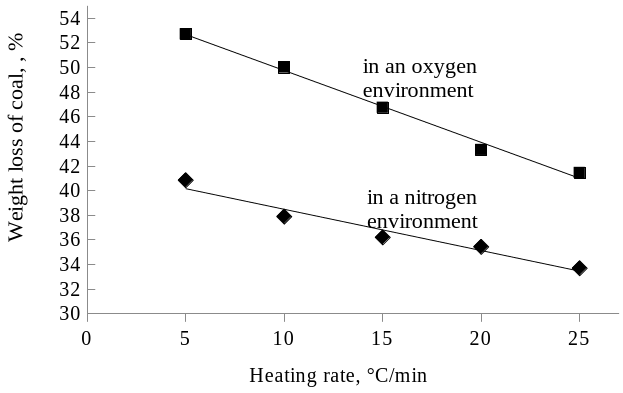
\includegraphics[width=0.6\textwidth]{assets/1086}
	\caption*{Figure 2 - Values of mass loss of coal samples at heating rates of 5-25 deg / min in nitrogen and oxygen environments}
\end{figure}

\begin{multicols}{2}
An increase in the heating rate β at all stages of OMC decomposition
leads to a shift in the temperature values T\textsubscript{max}
(corresponding to maximum decomposition) towards higher values, which
reflects an increase in the thermal stability of coal (Figure 3). So,
for a nitrogen environment, an increase in Тmax for the
1\textsuperscript{st} stage ΔТ\textsubscript{max} = 82 °С, for the
2\textsuperscript{nd} stage ΔТ\textsubscript{max} = 96 °С, for the
3\textsuperscript{rd} stage ΔТ\textsubscript{max} = 160 °С. For the
oxygen environment, the increase in Т\textsubscript{max} for the 1st
stage ΔТ\textsubscript{max} = 89 °С, the 2\textsuperscript{nd}stage
ΔТ\textsubscript{max} = 98 °С, the 3rd stage ΔТ\textsubscript{max} = 114
°С.
\end{multicols}

\begin{figure}[H]
	\centering
	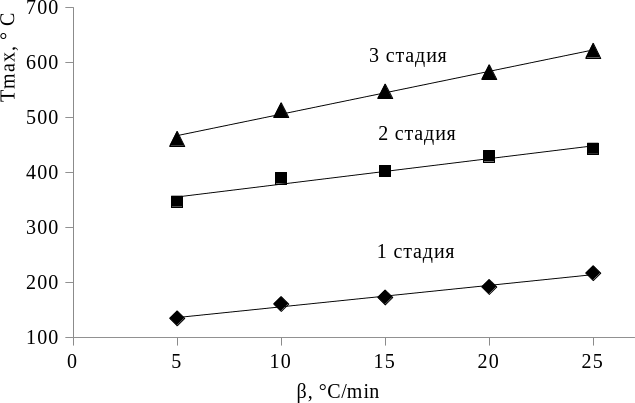
\includegraphics[width=0.6\textwidth]{assets/1087}
	\caption*{Figure 3 - Dependence of the temperature at the inflection points on the heating rate of coal at various stages of decomposition in a nitrogen environment}
\end{figure}

\begin{multicols}{2}
An increase in the heating rate β leads to an increase in the rate
v\textsubscript{max} of the OMC destruction process. At the same time,
the approximation of points by a straight line makes it possible to
obtain approximate relationships between v\textsubscript{max} and β
(Figure 4). At the same time, the difference between the speed
v\textsubscript{max} at the 1st stage and the speed v\textsubscript{max}
at the 2nd stage (ie the difference Δv\textsubscript{max} between the
velocities at the inflection points) also increases with increasing β.
This relationship between Δv\textsubscript{max} and β is described by a
similar function close to linear.
\end{multicols}

\begin{figure}[H]
	\centering
	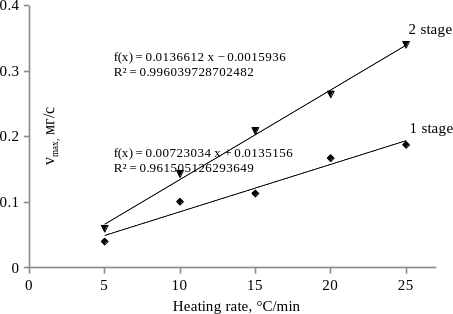
\includegraphics[width=0.6\textwidth]{assets/1088}
	\caption*{Figure 4 - Dependence of the rate of destruction at the inflection points on the rate of heating of coal at various stages of decomposition in a nitrogen environment}
\end{figure}

\begin{multicols}{2}
During the transition from one stage of the main decomposition to
another with an increase in temperature (over the entire range of β),
there is a noticeable increase in Е\textsubscript{act} (Tables 4, 5) and
k\textsubscript{0} (by 2 orders of magnitude, i.e. k\textsubscript{01}
\textasciitilde{} 10\textsuperscript{2} s\textsuperscript{-1},
k\textsubscript{02} \textasciitilde{} 10\textsuperscript{4}
s\textsuperscript{-1}), i.e. more and more stable molecular structures
are involved in the process of OMC destruction. But with an increase in
the heating rate β (within each stage of decomposition), the activation
energy Е\textsubscript{act} decreases.

The kinetic parameters of thermal destruction of Kenderlyk coal obtained
in this work are in good agreement with similar parameters for coals
from other Kazakh deposits {[}14-15{]}. In these works, the rate
constant k\textsubscript{max} (\textasciitilde10\textsuperscript{-3}
s\textsuperscript{-1}) and the pre-exponential factor k\textsubscript{0}
(\textasciitilde10\textsuperscript{2} s\textsuperscript{-1} and
\textasciitilde10\textsuperscript{4} s\textsuperscript{-1},
respectively, for the 1\textsuperscript{st} and 2\textsuperscript{nd}
stages of the main decomposition of OMC) have comparable values with
those for Kenderlyk coal, and the activation energy was in the range of
≈30-100 kJ/mol.

{\bfseries Conclusion.} Thus, the article reveals the dependence of the
kinetic parameters of the coal pyrolysis on the rate and temperature of
heating, describes the dependence between the kinetic parameters at
different stages of the main decomposition of coal. The kinetic
compensation effect is also established, the equations of linear
regression of the activation energy and the pre-exponential factor are
derived. The data obtained show that a longer thermolysis time has a
more significant effect on the coal degradation process than its heating
rate. It should be noted that the process of basic thermal decomposition
of OMC itself can be approximately described by the equation of formal
kinetics of the 1st order, i.e. the equation of monomolecular
transformation, since the exponents of the process under study vary
within ≈1.0-1.2 {[}15{]}. In general, it can be noted that the
calculated values of the activation energy of the stages of the main
thermal decomposition of coal are commensurate with the energies of
chemical bonds.

\emph{{\bfseries Financing.} This work was carried out with financial
support from the Science Committee of the Ministry of Science and Higher
Education of the Republic of Kazakhstan (No. BR21882171 "SDG 9.4:
Development of the "green" economy of Kazakhstan through the processing
of mineral raw materials and waste by pyrolysis").}

Авторы выражают благодарность за выделенное грантовое финансирование.
\end{multicols}

\begin{center}
{\bfseries References}
\end{center}

\begin{noparindent}
1.Sangcheol Shin, Soo Ik Im, Nam Sun Nho, Ki Bong Lee. Kinetic analysis
using thermogravimetric analysis for nonisothermal pyrolysis of vacuum
residue //Journal of Thermal Analysis and Calorimetry, 2016.-Vol.126.-
P.933--941. http://doi.org/10.1007/s10973-016-5568-6.

2.Xu Y., Zhang Y., Wang Y., Zhang G., Chen L. Thermogravimetric study of
the kinetics and characteristics of the pyrolysis of lignite //Reaction
Kinetics, Mechanisms and Catalysis, 2013. -- Vol. 110.- P.225--235.

http://doi.org/10.1007/s11144-013-0586-x

3.Mar\textquotesingle jandyshev P.A., Chernov A. A., Popova E. I.,
Ljubov V. K. Issledovanie processa termicheskogo razlozhenija i gorenija
uglej, drevesnogo topliva i gidroliznogo lignina termicheskimi metodami
analiza //Himija tverdogo topliva,2016 - № 3.- S.30-39.

http://doi.org/10.7868/S0023117716030099 {[}in Russ.{]}.

4.Czajka K., Kisiela A., Moroń W., Ferens W., Rybak W. Pyrolysis of
solid fuels: Thermochemical behaviour, kinetics and compensation effect
//Fuel Processing Technology, 2016. -Vol. 142.- P.42--53.

http://dx.doi.org/10.1016/j.fuproc.2015.09.027

5.Godois Baroni E., Tannous K., Rueda-Ordycez Y. J., Tinoco-Navarro L.
K. The applicability of isoconversional models in estimating the kinetic
parameters of biomass pyrolysis //Journal of Thermal Analysis and
Calorimetry, 2016.- Vol.123.- P.909 - 917.

http://dx.doi.org/10.1007/s10973-015-4707-9

6.Kozlov A.N., Svishchev D.A., Khudiakova G.I., Ryzhkov A.F. A kinetic
analysis of the thermochemical

conversion of solid fuels (A review) //
Solid Fuel Chemistry, 2017. -- Vol. 51: 205-213

http://dx.doi.org/10.3103/S0361521917040061

7.Bojko E.A., S.V. Pachkovskij, D. G. Didichin.
Jeksperimental\textquotesingle no-raschetnaja metodika ocenki
kineticheskih processov termohimicheskogo prevrashhenija tverdyh
organicheskih topliv // Fizika gorenija i vzryva, 2005. - №1.- S. 55-65
{[}in Russ.{]}.

8.Shishmarev P.V., Bojko E.A., Pachkovskij S.V. Kompleksnyj termicheskij
analiz. Sovershenstvovanie i vnedrenie v praktiku jenergeticheskogo
ispol\textquotesingle zovanija Kansko-Achinskih uglej //LAMBERT Akademik
Publishing

(Germanija), 2012. - 250 s. {[}in Russ.{]}.

9.Du Z., Sarofim A.F., Longwell J.P. Activation Energy Distribution in
Temperature Programmed Desorption: Modeling and Application to the Soot
Oxygen System //Energy \& Fuels, 1990.- Vol. 4(3).- P. 296--302.

http://doi.org/10.1021/ef00021a014

10.Du Z., Sarofim A. F., Longwell J. P., Mims C. A. Kinetic Measurement
and Modeling of Carbon Oxidation // Energy and Fuels, 1991. -Vol.5(1)-
P.214-221.

http://doi.org/10.1021/ef00025a035 {[}in Eng.{]}.

11.Gjul\textquotesingle maliev A.M., Golovin G.S., Gladun T.G.
Teoreticheskie osnovy himii uglja. M.: Izdatel\textquotesingle stvo
Moskovskogo gosudarstvennogo gornogo universiteta, 2003.-556 s. ISBN:
5-7418-0243-5 {[}in Russ.{]}.

12.Shevkopljas V.N. Raschet osnovnyh kineticheskih parametrov tverdyh
topliv po dannym derivatograficheskogo analiza // Voprosy himii i
himicheskoj tehnologii, 2007.-№ 2.- S.179-183 {[}in Russ.{]}.

13.Faljushin P.L. Dudarchik V.M., Krajko V.M., Anufrieva E.V.,
Smoljachkova E.A. Termoustojchivost\textquotesingle{} buryh uglej
Lel\textquotesingle chickogo mestorozhdenija //
Prirodopol\textquotesingle zovanie, 2012.- Vypusk 21.- S. 305-311 {[}in
Russ.{]}.

14.Bekturganov N.S., Yermagambet B.T., Kassenov B.K., Nurgaliyev N.U.,
Nabiyev M.A., Kassenova Zh.M., Aibuldinov Ye.K., Bizhanova L.N. Research
of kinetics of thermal decomposition of coal of Kazakhstani deposit//
CPSI Journal (a magazine by the coal preparation society of India),
2015.-Vol.(19).- P.17-21.

15.Nabiev M.A., Ermagambet B.T., Bekturganov N.S., Nurgaliyev N.U.,
Kasenova Zh.M., Bizhanova L.N. Kinetika termodestrukcii uglja
Shubarkol\textquotesingle skogo mestorozhdenija, Sb. st. «Innovacii v
nauke» po materialam LI mezhdunar. nauchno-prakt. konf. − Ser.
Tehnicheskie nauki, Novosibirsk, 2015. -- No.11 (48). -- Ch. I. -- S.
156-161 {[}in Russ.{]}.
\end{noparindent}

\emph{{\bfseries Information about the authors}}

\begin{noparindent}
Nurgaliyev N. U.- Candidate of Chemical Science, Associate
Professor,Kazakh University of Technology and Business named after K.
Kulazhanov, Astana, Kazakhstan, Astana, e-mail: nurgaliev\_nao@mail.ru;

Aybuldinov E. K.-PhD, Research Institute of New Chemical Technologies,
L.N. Gumilyov Eurasian National University, Astana, Kazakhstan, e-mail:
elaman\_@mail.ru;

Iskakova Zh. B.- Candidate of Chemistry Sciences, Associate Professor,
Research Institute of New Chemical Technologies, L.N. Gumilyov Eurasian
National University, Astana Kazakhstan, e-mail: zhanariskakova@mail.ru;

Kolpek A.- Candidate of Chemistry Sciences, Associate Professor, L.N.
Gumilyov Eurasian National University, Astana, Kazakhstan, e-mail:
aynagulk@mail.ru;

Mashan T. T.-Candidate of Chemical Sciences, Associate Professor, L.N.
Gumilyov Eurasian National University, Astana, Kazakhstan, e-mail:
togzhan-mashan@mail.ru4

Kusepova L. A.- Candidate of Chemical Sciences, Associate Professor,
L.N. Gumilyov Eurasian National

University, Astana, Kazakhstan, e-mail:
kusepova71@mail.ru

Kopishev E. Ye. -Candidate of Chemistry Sciences, L.N. Gumilyov Eurasian
National University, Astana,

Kazakhstan, e-mail: eldar\_kopishev@mail.ru
\end{noparindent}

\emph{{\bfseries Сведения об авторах}}

\begin{noparindent}
Нургалиев Н. У.- кандидат химических наук, ассоциированный профессор,
Казахский университет технологии и бизнеса имени К.Кулажанова, Астана,
Казахстан, e-mail: nurgaliev\_nao@mail.ru;

Айбульдинов Е.К.- доктор PhD, Научно-исследовательский институт Новых
химических технологий, Евразийский национальный университет им. Л.Н.
Гумилева, Астана, Казахстан, e-mail: elaman\_@mail.ru;

Искакова Ж. Б.-кандидат химических наук, ассоциированный профессор,
Научно-исследовательский институт Новых химических технологий,
Евразийский национальный университет им. Л.Н. Гумилева, Астана,
Казахстан, e-mail: zhanariskakova@mail.ru;

Колпек А.- кандидат химических наук, ассоциированный профессор, кафедра
химии, факультет естественных наук, Евразийский национальный университет
им. Л.Н. Гумилева, Республика Казахстан, г. Астана, e-mail:
aynagulk@mail.ru;

Машан Т.Т.-кандидат химических наук, доцент, кафедра химии, факультет
естественных наук, Евразийский национальный университет им. Л.Н.
Гумилева, Астана, Казахстан, e-mail: togzhan-mashan@mail.ru;

Кусепова Л.А. -кандидат химических наук, доцент, Евразийский
национальный университет им. Л.Н. Гумилева, Астана Казахстан, , e-mail:
kusepova71@mail.ru;

Копишев Э. Е.-кандидат химических наук, Евразийский национальный
университет им. Л.Н. Гумилева, Астана, Казахстан, e-mail:
eldar\_kopishev@mail.ru
\end{noparindent}
